\documentclass[11pt,a4paper]{article}

\usepackage{fontspec}
\usepackage{microtype}
\usepackage[margin=2.5cm]{geometry}
\usepackage{amsmath,amssymb}
\usepackage{booktabs,tabularx,array}
\usepackage{enumitem}
\usepackage{caption}
\usepackage{graphicx}
\usepackage{tikz}
\usetikzlibrary{positioning,arrows.meta,calc}
\usepackage[hidelinks]{hyperref}

\captionsetup{font=small,labelfont=bf}
\setlist{itemsep=2pt,topsep=4pt}
\newcolumntype{L}{>{\raggedright\arraybackslash}X}
\newcolumntype{C}{>{\centering\arraybackslash}X}
\newcommand{\code}[1]{\texttt{#1}}
\newcommand{\ms}{\,\mathrm{ms}}
\renewcommand{\arraystretch}{1.15}
\setlength{\emergencystretch}{2em}

\title{P-Wave Detection on a Mixed Pool of Non-12-Lead ECG\\
\large Rules, Logistic Regression and CNN Candidate Features on a New Patient-Wise Split}
\author{Emanuel Bierschneider}
\date{November 2026}

\begin{document}
\maketitle

\begin{abstract}
\noindent
Two prior studies constructed and refined a P-wave detector for single-lead ECG sampled at 128\,Hz. The detector combines a rule-based front end with a logistic-regression (LR) scorer over 22 hand-crafted candidate features, and, since the second study, two additional features produced by a small convolutional network (CNN) that examines the raw waveform around each candidate. Both studies relied on a single fixed split over four databases, one of which is 12-lead (LUDB).

The present paper evaluates the detector on a new data pool. Every available non-12-lead ECG was pooled: the labelled databases BUT PDB, PhysioNet PWAVE and QTDB (335 files, 61,338 lead-wise P labels) together with 247.5\,h of unlabelled single-lead ECG (Icentia11k, PhysioNet/CinC 2017, BUT QDB). A fresh patient-wise split was drawn over the pooled patient groups using a salt fixed in advance. The rule parameters, the scorer and the CNNs were fitted on the training patients, and every choice was made on validation. The test split was scored once.

\medskip
\begin{center}
\begin{tabular}{lccc}
\toprule
Detector (macro $F_1$ over 3 databases) & Train & Validation & Test \\
\midrule
Rules (tuned) & 87.64\,\% & 86.42\,\% & 82.87\,\% \\
Rules + LR, 22 features & 88.64\,\% & 89.21\,\% & 90.58\,\% \\
Rules + LR + 3-CNN ensemble & 92.75\,\% & 91.57\,\% & 91.45\,\% \\
\bottomrule
\end{tabular}
\end{center}
\medskip

The conclusions of the earlier studies carried over to the new pool. The learned scorer provides the largest improvement over the rules ($+2.79$ points $[+1.06, +5.58]$ on validation, $+7.71$ $[+5.43, +11.88]$ on test, paired patient bootstrap). The CNN features contribute $+2.35$ $[+1.10, +4.08]$ on validation and $+0.87$ $[-0.09, +2.00]$ on test. FixMatch with 50\,h of unlabelled ECG did not outperform supervised CNN training (91.36\,\% vs.\ 91.57\,\% on validation), and boosted trees overfitted. In atrial fibrillation the CNN reduced false P detections on validation from 12.3 to 6.7 per 100 beats. The test split turned out to be small (8.8\,\% of the P labels, a single PWAVE patient), so its numbers are less reliable than those on validation.
\end{abstract}

% ------------------------------------------------------------------
\section{Data}
\label{sec:data}

\paragraph{The pool.} Table~\ref{tab:pool} lists every non-12-lead dataset that was available. The labelled files are JSON files carrying P and QRS peak positions, together with AF rhythm intervals wherever the source provides them. Each file stores the native signal and a 128\,Hz copy. The 335 labelled files all reside in a single folder. A file's database is inferred from its name solely for the purpose of reporting results per database. Each lead of a labelled file is handled as an independent single-lead recording with its own labels.

\begin{table}[ht]
\centering
\caption{The non-12-lead pool. P labels are counted per lead. LUDB (200 files, 12 leads) was excluded.}
\label{tab:pool}
\begin{tabularx}{\linewidth}{lLrrrr}
\toprule
Dataset & Content & Files & Groups & Hours & P labels \\
\midrule
BUT PDB \cite{butpdb} & 2-min Holter excerpts from MIT-BIH, SVDB and LTAFDB; rich in pathology & 50 & 45 & 1.7 & 10,858 \\
PWAVE \cite{pwave} & 12 MIT-BIH Arrhythmia records \cite{mitbih}, each cut into 15 files of 2\,min & 180 & 12 & 6.0 & 44,092 \\
QTDB \cite{qtdb} & Annotated sections of 105 records; only selected beats labelled & 105 & 105 & 2.2 & 6,388 \\
\midrule
Icentia11k \cite{icentia} & Chest patch, middle 70\,min of 100 outpatients & 100 & 100 & 116.5 & -- \\
CinC 2017 \cite{cinc2017} & AliveCor handheld, 9--61\,s recordings & 8,528 & 8,528 & 77.0 & -- \\
BUT QDB \cite{butqdb} & Wearable, everyday activity, 3\,h of 18 recordings & 54 & 15 & 54.0 & -- \\
\midrule
Total & & 9,017 & 8,785 & 257.4 & 61,338 \\
\bottomrule
\end{tabularx}
\end{table}

\paragraph{What the data contain and what not.} Table~\ref{tab:content} summarises what each kind of file provides. In brief, the labelled files supply ECG signal, P-peak positions, QRS positions and a coarse AF/non-AF rhythm label. They provide no P-wave boundaries, no other waves and no clinical information. The unlabelled files provide nothing but the ECG signal.

\begin{table}[ht]
\centering
\caption{What the data used in this paper contain (\checkmark) and do not contain (--).}
\label{tab:content}
\small
\begin{tabularx}{\linewidth}{Lcc}
\toprule
Content & Labelled (BUT PDB, PWAVE, QTDB) & Unlabelled (Icentia11k, CinC 2017, BUT QDB) \\
\midrule
ECG signal at native rate and at 128\,Hz & \checkmark & \checkmark{} (resampled when read) \\
Number of leads & 2 & 1 \\
P-wave \emph{peak} positions, per lead & \checkmark & -- \\
P-wave onset and offset, P shape class & -- & -- \\
QRS positions (one time per beat) & \checkmark & -- (R peaks detected) \\
Beat type (normal, ventricular, \ldots) & -- & -- \\
T waves, PR / QT intervals & -- & -- \\
Rhythm intervals: AF vs.\ other & \checkmark & -- (not copied) \\
Finer rhythm classes (flutter, AV block, \ldots) & -- (``other'') & -- \\
Every beat annotated & \checkmark{} (QTDB: selected beats) & -- \\
Signal-quality labels & -- & -- (not copied) \\
Patient identity & group of the source patient & per file or per subject \\
Age, sex, diagnosis, medication & -- & -- \\
\bottomrule
\end{tabularx}
\end{table}

Several details matter for the results:
\begin{itemize}
\item \textbf{Labels are positions, not waveforms.} A P label is a single time point, the peak of the P wave, placed by the human annotators of each database. The detector is therefore judged only on where it places the peak ($\pm50\ms$), not on P duration or shape.
\item \textbf{Labels are per lead.} The two leads of a labelled file each carry their own P labels. A P wave that is visible in only one lead is labelled in that lead alone. Both leads originate from the same heartbeats, so they are not independent samples.
\item \textbf{Labels are absent where there is no P wave.} In AF, and in beats where the annotators saw no P wave, no label exists. A detection there counts as false. AF intervals are labelled in all three databases where the source carries rhythm annotations; most AF beats are in BUT PDB.
\item \textbf{QTDB labels only selected beats} (roughly 30 per record). Detections outside those beats are neither right nor wrong and are ignored.
\item \textbf{The unlabelled sources had labels in their original releases} (Icentia11k beat and rhythm labels, CinC 2017 rhythm classes, BUT QDB signal quality). None of these was copied; the CNN only ever sees their raw signal.
\end{itemize}

\paragraph{Shared patients.} BUT PDB, PWAVE and QTDB all include excerpts of MIT-BIH patients. Each file is therefore mapped to a \emph{patient group} that names its source patient (for example \code{mitdb:231}). 19 groups occur in more than one labelled database: 8 in BUT PDB and QTDB, 6 in BUT PDB and PWAVE, 4 in PWAVE and QTDB, and 1 in all three. The 180 PWAVE files originate from only 12 patients.

\paragraph{Split.} Every labelled patient group is assigned to train, validation or test with probability 60\,/\,20\,/\,20\,\%. The assignment is a hash of \code{mixed-v1:<group>}. The groups of all databases are pooled, so the split is not stratified by database. The salt \code{mixed-v1} was fixed before any result was seen; it was only checked afterwards that every database occurs in every split. No group lies in more than one split. The unlabelled data are used only for training (FixMatch) and do not overlap with the labelled databases.

\begin{table}[ht]
\centering
\caption{The new split: files (patient groups) and lead-wise P labels.}
\label{tab:split}
\begin{tabular}{lccc}
\toprule
Database & Train & Validation & Test \\
\midrule
BUT PDB & 32 (28), 7,916 & 11 (10), 1,812 & 7 (7), 1,130 \\
PWAVE & 120 (8), 31,244 & 45 (3), 9,842 & 15 (1), 3,006 \\
QTDB & 69 (69), 4,122 & 16 (16), 1,030 & 20 (20), 1,236 \\
\midrule
Patient groups & 92 & 25 & 25 \\
P labels & 43,282 (70.6\,\%) & 12,684 (20.7\,\%) & 5,372 (8.8\,\%) \\
\bottomrule
\end{tabular}
\end{table}

Table~\ref{tab:split} shows the outcome. Because the split is random over patients and PWAVE has few patients with many labels each, the split is uneven in labels. Train holds 70.6\,\% of the P labels, test only 8.8\,\%. The PWAVE part of test is a single patient (15 files). This was accepted rather than redrawn, since redrawing after seeing the split would be a choice made on the data.

\paragraph{Metric.} A detection matches a reference P peak within $\pm50\ms$, one-to-one. Sensitivity (Se), positive predictive value (PPV) and $F_1$ are computed per database. In QTDB, where only selected beats are labelled, only detections inside annotated beats are scored. The headline number is the \emph{macro} $F_1$, the mean of the three per-database $F_1$ values, so PWAVE does not dominate. It is used for every choice. The \emph{pooled} $F_1$, which counts all files as one dataset, is reported alongside. Confidence intervals come from a patient bootstrap ($B = 2000$). Differences between detectors are paired: both are scored on the same resampled patients.

% ------------------------------------------------------------------
\section{Methods}

The detector is that of the earlier studies \cite{prev,prevcnn}; this section summarises it.

\begin{figure}[ht]
\centering
\resizebox{\linewidth}{!}{%
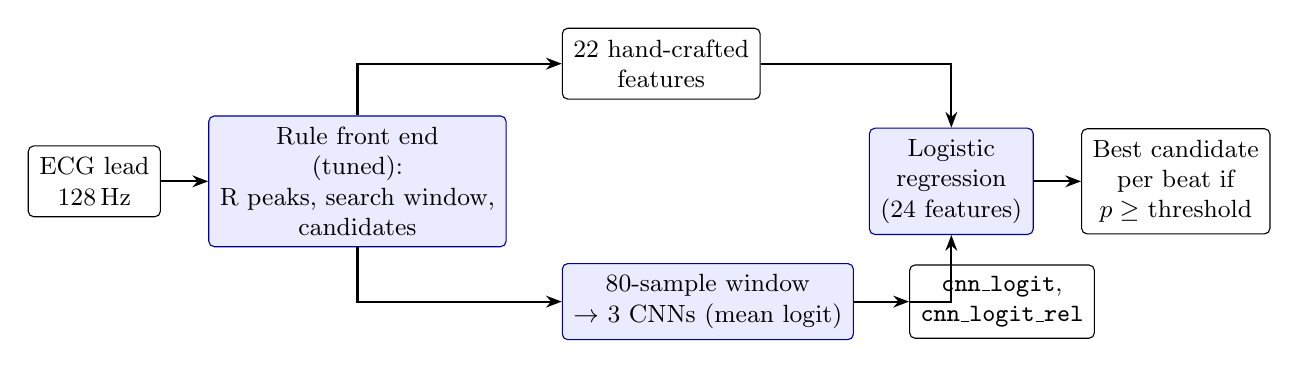
\begin{tikzpicture}[
  box/.style={draw, rounded corners=2pt, align=center, font=\small, minimum height=0.9cm, inner sep=4pt},
  new/.style={box, fill=blue!8, draw=blue!60!black},
  arr/.style={-{Stealth[length=2mm]}, thick}]
\node[box] (ecg) {ECG lead\\128\,Hz};
\node[new, right=0.6cm of ecg] (front) {Rule front end\\(tuned):\\R peaks, search window,\\candidates};
\node[box, above right=0.2cm and 0.7cm of front] (feat) {22 hand-crafted\\features};
\node[new, below right=0.2cm and 0.7cm of front] (win) {80-sample window\\$\rightarrow$ 3 CNNs (mean logit)};
\node[box, right=0.7cm of win] (cnnf) {\code{cnn\_logit},\\\code{cnn\_logit\_rel}};
\node[new, right=4.6cm of front] (lr) {Logistic\\regression\\(24 features)};
\node[box, right=0.6cm of lr] (dec) {Best candidate\\per beat if\\$p \ge$ threshold};
\draw[arr] (ecg) -- (front);
\draw[arr] (front) |- (feat);
\draw[arr] (front) |- (win);
\draw[arr] (win) -- (cnnf);
\draw[arr] (feat) -| (lr);
\draw[arr] (cnnf) -| (lr);
\draw[arr] (lr) -- (dec);
\end{tikzpicture}}
\caption{The detector. Shaded parts were tuned or fitted on the training patients.}
\label{fig:pipeline}
\end{figure}

All filters are Butterworth filters applied forwards and backwards (zero phase). All signals are at 128\,Hz; the labelled files contain a 128\,Hz channel, and unlabelled signals are resampled to 128\,Hz with a polyphase filter.

\subsection{Rule front end}
\label{sec:front}

\paragraph{Pre-processing.} Each lead is band-pass filtered at 0.5--40\,Hz (order 2) to remove baseline wander and high-frequency noise. This signal $x_f$ is the reference for amplitudes and for the R-peak positions.

\paragraph{R peaks (Elgendi detector \cite{elgendi2013}).} The raw lead is band-pass filtered at 8--20\,Hz (order 3), where the QRS complex has most of its energy, and squared. Two moving averages of the squared signal are formed, one over 97\,ms (about one QRS width) and one over 611\,ms (about one beat). Wherever the short average exceeds the long average plus $0.08$ times the mean of the squared signal, a \emph{block of interest} begins. Blocks shorter than 97\,ms are discarded. In each remaining block, the R peak is the largest absolute value of $x_f$. The dominant QRS polarity of the lead is the sign of the median R amplitude; within $\pm50\ms$ of each peak the extremum with that sign replaces the absolute maximum, unless it is smaller than 30\,\% of it. Of two peaks closer than 250\,ms (refractory period), the larger is kept.

\paragraph{QRS onset and offset.} A QRS energy envelope is formed by band-passing at 8--20\,Hz, squaring and a 40\,ms moving average. From the maximum of the envelope near R, the onset is found by walking back until the envelope falls below 10\,\% of that maximum (parameter \code{onset\_frac}), at most 200\,ms. The offset is found the same way forwards.

\paragraph{QRS blanking and P band.} In a copy of $x_f$, every QRS complex from onset to offset is replaced by a straight line between its end points. This copy is low-pass filtered at 15\,Hz (order 2, parameter \code{p\_lp}) to give the \emph{P-band signal} $x_p$. Without the blanking, the low-pass would smear QRS energy into the PR segment and create false peaks just before the QRS.

\paragraph{Search window.} For each beat, the P search window runs from 300\,ms before R to 8\,ms before the QRS onset (parameter \code{guard}). It never starts earlier than 120\,ms after the previous R peak, so it cannot reach into the previous QRS. Beats with a window shorter than 3 samples are skipped.

\paragraph{Lead template and P polarity.} The P-band segments of the 400\,ms before every R peak are aligned on R, each minus its median, and their sample-wise median forms the lead's \emph{P template}. Its most prominent peak inside the typical search window gives the lead's P polarity and the typical P latency (time from P peak to R). A negative peak is chosen only if its prominence is 3 times that of the best positive peak (parameter \code{neg\_bias}), because small negative deflections in the PR segment are common. The template snippet of $\pm60\ms$ around its peak is kept for shape comparison.

\paragraph{Candidates.} A \emph{candidate} is a possible P-wave peak, never the R peak. Every local maximum of the polarity-corrected P-band signal inside the search window is a candidate (Python \code{scipy.signal.find\_peaks}). For each candidate three numbers are computed:
\begin{itemize}
\item its \emph{prominence}, the height above the higher of the two surrounding minima, computed with 100\,ms of extra context to the left of the window;
\item its \emph{shape correlation}, the Pearson correlation of the $\pm60\ms$ around it with the template snippet;
\item its \emph{noise floor}. The high-frequency noise of a beat is the robust standard deviation ($1.4826 \times$ median absolute deviation) of the 0.5--40\,Hz signal minus the 0.5--15\,Hz signal inside the window, smoothed as the median over $\pm8$ beats. The low-frequency activity is the robust standard deviation of $x_p$ in the window without the $\pm50\ms$ around the candidate. The noise floor is $\sqrt{\text{hf}^2 + (0.5\,\text{lf})^2}$.
\end{itemize}
A beat has 1.8 candidates on average. One of them is often the true P peak; the others are noise bumps, the tail of the previous T wave, notches in the PR segment, or ripples in atrial fibrillation.

\paragraph{Rule decision.} The rule detector picks one candidate per beat in two passes.
\begin{enumerate}
\item \textbf{Global latency prior.} Each candidate's prominence is multiplied by a Gaussian of its latency around the template latency ($\sigma = 30\ms$). The highest-scoring candidate is accepted if its prominence is at least $k$ times the noise floor ($k = 1$), at least an amplitude minimum, and its shape correlation is at least 0.7. The amplitude minimum is $\min(0.015 \cdot A_R,\ 0.02)$, where $A_R$ is the lead's median absolute R amplitude.
\item \textbf{Beat-to-beat consistency.} The PR latency is nearly constant from beat to beat in sinus rhythm. For each beat, the median latency of the candidates accepted in pass 1 among the 4 neighbouring beats on each side is formed. If at least 2 neighbours give a latency, the candidate is chosen with a narrower prior ($\sigma = 25\ms$) around it, must lie within 40\,ms of it, and the thresholds of pass 1 are relaxed by the factor 0.6. If fewer neighbours exist, the template prior is used and the prominence must be at least twice the noise floor.
\end{enumerate}
The position of an accepted peak is refined to sub-sample accuracy by fitting a parabola through the peak sample and its two neighbours. An optional ectopy gate suppresses P waves in beats whose QRS ($\pm60\ms$ around R) correlates less than 0.7 with the lead's median QRS; tuning switched it off (below).

\subsection{Rule tuning}

The 24 rule parameters start from fixed values. 17 of them have a grid of 3 to 5 values each (Table~\ref{tab:grid}). Coordinate descent goes through the parameters in a fixed order. For each, every grid value is tried with all other parameters fixed, and a value is kept if the training macro $F_1$ rises by at least 0.1 points; smaller gains are treated as noise. One pass over all parameters is a round. After each of two rounds the validation macro $F_1$ is computed, and the round with the higher value is kept.

\begin{table}[ht]
\centering
\caption{Rule parameters tuned by coordinate descent, their grids and the chosen values. Changed values in bold.}
\label{tab:grid}
\small
\begin{tabularx}{\linewidth}{lLll}
\toprule
Parameter & Meaning & Grid & Chosen \\
\midrule
\code{min\_amp\_rel} & amplitude minimum relative to $A_R$ & 0.005, 0.01, 0.015, 0.02 & \textbf{0.015} (start 0.01) \\
\code{amp\_cap} & upper cap of the amplitude minimum & 0.01 \ldots\ 0.03, none & 0.02 \\
\code{k\_noise} & prominence / noise floor & 0.5, 1, 1.5, 2, 3 & 1.0 \\
\code{relax} & threshold factor for consistent beats & 0.4 \ldots\ 1.0 & 0.6 \\
\code{min\_corr} & minimum template correlation & 0.4 \ldots\ 0.8 & 0.7 \\
\code{k\_isolated} & prominence / noise without neighbours & 1.5, 2, 3, 5, off & 2.0 \\
\code{nb\_tol}, \code{nb\_sigma} & tolerance and prior width around the local latency & 15--60\,ms & 40, 25\,ms \\
\code{nb\_beats}, \code{nb\_min} & neighbours per side, minimum used & 2--6, 1--3 & 4, 2 \\
\code{qrs\_corr\_min} & ectopy gate & off, 0.5, 0.7, 0.8 & \textbf{off} (start 0.7) \\
\code{lat\_sigma} & width of the template latency prior & 20, 30, 45\,ms & 30\,ms \\
\code{p\_lp} & P-band low-pass & 10, 12, 15, 20\,Hz & 15\,Hz \\
\code{guard} & gap before QRS onset & 8, 16, 30\,ms & 8\,ms \\
\code{neg\_bias} & preference for positive P & 1.5, 3, 5 & 3 \\
\code{lf\_weight} & weight of low-frequency activity in the noise floor & 0, 0.5, 1 & 0.5 \\
\code{onset\_frac} & QRS onset threshold & 0.05, 0.10, 0.15 & 0.10 \\
\bottomrule
\end{tabularx}
\end{table}

Training macro $F_1$ rose from 87.19\,\% to 87.64\,\% in round 0 (validation 86.42\,\%); round 1 changed nothing. Each evaluation of one parameter set on the training patients takes about 25\,s. The tuned values are stored in \code{tuned\_params.json} and used by every later step, both for the rule detector and as the front end of the learned detectors.

\subsection{Candidate features and learned scorer}

\paragraph{Features.} The learned detectors use the same candidates as the rules, but replace the rule decision by a classifier. Every candidate is described by 22 features (Table~\ref{tab:feat}). They express what the rules use as thresholds (prominence, noise, correlation, latency) as continuous values, and add context the rules use only implicitly: the other candidates of the beat, the neighbouring beats and the heart rhythm.

\begin{table}[ht]
\centering
\caption{The 22 candidate features. ``Latency'' is the time from candidate to R; $A_R$ is the lead's median R amplitude; nf the candidate's noise floor.}
\label{tab:feat}
\small
\begin{tabularx}{\linewidth}{lL}
\toprule
Group & Features \\
\midrule
Amplitude (3) & $\log(\text{prominence}/\text{nf})$, $\log(\text{prominence}/A_R)$, $\log(\text{prominence})$ \\
Shape (1) & correlation with the template snippet \\
Latency (3) & latency; $|$latency $-$ template latency$|$; $|$latency $-$ median accepted latency of $\pm4$ neighbouring beats$|$ \\
Neighbours (2) & whether any neighbour has an accepted P; share of neighbours with one \\
Within the beat (3) & rank by prominence; prominence / largest prominence of the beat; number of candidates \\
Window (3) & distance to window start, to window end; window length \\
QRS (1) & correlation of the beat's QRS with the lead's median QRS (ectopy) \\
Noise (1) & $\log(\text{nf}/A_R)$ \\
Rhythm (4) & previous and next RR interval / median RR; their ratio; median absolute RR change over $\pm4$ beats / median RR (irregularity, high in AF) \\
Lead (1) & $\log$(template prominence / median noise floor), the quality of the lead's P template \\
\bottomrule
\end{tabularx}
\end{table}

\paragraph{Training rows and labels.} Every candidate of a training lead is a row. Its label is 1 if a reference P peak lies within $\pm50\ms$, else 0. Only candidates inside the labelled time range are used, and in QTDB only candidates of annotated beats (R within 80\,ms of an annotated QRS). Rows are weighted so that each database has the same total weight, matching the macro objective; otherwise PWAVE would provide 72\,\% of the training P labels.

\paragraph{Scorers.} Four scorers were fitted with scikit-learn \cite{sklearn}:
\begin{itemize}
\item \textbf{Logistic regression}: features standardised to zero mean and unit variance, L2 penalty with $C = 1$.
\item \textbf{Histogram gradient-boosted trees} in three sizes: small (depth 3, 200 trees, learning rate 0.1), medium (depth 5, 300 trees, 0.05, at least 50 rows per leaf) and large (depth 8, 400 trees, 0.05, at least 100 rows per leaf), all with L2 regularisation 1.
\end{itemize}

\paragraph{Decision.} In each beat the candidate with the highest probability is taken, and it is reported if its probability is at least a threshold. The threshold is chosen from $\{0.2, 0.3, \ldots, 0.7\}$ on validation, jointly with the scorer. The reported position is refined by the same parabola fit as in the rules. Because at most one candidate per beat is reported, a beat cannot produce two detections.

\subsection{CNN candidate features}

\paragraph{Window.} For every candidate, 80 samples (625\,ms) of the 128\,Hz lead are cut from 40 samples before to 39 samples after it; at the signal edges the signal is padded with its edge value. The window is taken from the raw lead, not from the P-band signal, so the CNN sees the waveform as recorded. Its median is subtracted, it is divided by $A_R$ (here the median absolute R value after removing the lead's median), and it is clipped to $\pm10$. A true P peak lies 100--250\,ms before R, so its window shows the whole P wave, the PR segment, the QRS complex and part of the ST segment. Where the QRS appears in the window tells the network the candidate's distance to the QRS.

\paragraph{Network.} Table~\ref{tab:net} lists the layers. The output of the convolutions is flattened rather than pooled, because the position of a shape relative to the window centre matters. The network has 19,921 weights.

\begin{table}[ht]
\centering
\caption{CNN architecture. Each convolution is followed by batch normalisation and ReLU.}
\label{tab:net}
\small
\begin{tabular}{llll}
\toprule
Layer & Kernel, stride & Output channels & Output length \\
\midrule
Input & & 1 & 80 \\
Conv 1 & 7, 1 & 16 & 80 \\
Conv 2 & 5, 2 & 32 & 40 \\
Conv 3 & 5, 2 & 32 & 20 \\
Conv 4 & 3, 1 & 16 & 20 \\
Flatten, dropout 0.2 & & & 320 \\
Dense + ReLU & & & 32 \\
Dense (logit) & & & 1 \\
\bottomrule
\end{tabular}
\end{table}

\paragraph{Training.} The network is implemented in PyTorch \cite{pytorch}. The loss is binary cross-entropy with the same row labels and database weights as the LR. Training runs for 15 epochs with batch size 256 and AdamW (learning rate $10^{-3}$, weight decay $10^{-4}$) under a one-cycle schedule with peak learning rate $3\cdot10^{-3}$. After every step an \emph{exponential moving average} (EMA) of the weights is updated with decay 0.99; this averaged network, not the last state, is kept. It is smoother than any single step and serves as the teacher in FixMatch.

\paragraph{Window augmentation.} Each labelled batch is augmented. Each of four transforms is applied to a random half of the windows, with random strengths from the ranges in Table~\ref{tab:aug}:
\begin{itemize}
\item \textbf{Down- and up-sampling}: anti-aliased downsampling by a factor $f$, then linear interpolation back to 80 samples. This removes fine detail, as a lower sampling rate or a smoother recording would, without moving the P peak. Time reversal, used by ECGMatch \cite{ecgmatch}, is not used, because it would place the QRS before the P wave.
\item \textbf{Gain}: multiplication by a random factor, as from a different electrode position.
\item \textbf{Linear trend}: a ramp from $-a$ to $+a$ of random sign, imitating baseline wander.
\item \textbf{Gaussian noise} of standard deviation $\sigma$, imitating muscle noise.
\end{itemize}
None of the transforms moves the candidate, so the label stays valid.

\begin{table}[ht]
\centering
\caption{Augmentation ranges, in units of $A_R$ for trend and noise. ``Weak'' is used for labelled windows and the FixMatch teacher, ``strong'' for the FixMatch student.}
\label{tab:aug}
\small
\begin{tabular}{lcccc}
\toprule
& Resampling factor $f$ & Gain & Trend $a$ & Noise $\sigma$ \\
\midrule
Weak & 1.2--1.6 & 0.8--1.25 & 0--0.1 & 0.01--0.03 \\
Strong & 1.6--2.5 & 0.5--2.0 & 0.1--0.3 & 0.03--0.08 \\
\bottomrule
\end{tabular}
\end{table}

\paragraph{Ensemble.} Wherever a network is trained, three networks with different random seeds (initial weights, batch order, augmentation) are trained, and their logits are averaged. Averaging reduces the variance of a single small network trained on few patients.

\paragraph{Two CNN features.} The ensemble's logit $z$, clipped to $\pm10$, enters the LR as \code{cnn\_logit}. The second feature, \code{cnn\_logit\_rel} $= z - \max_{\text{beat}} z$, is 0 for the beat's best candidate by CNN and negative for the others. Because the detector reports only the best candidate per beat, this relative score matters as much as the absolute one. The LR then has 24 features and is fitted as above; its threshold is chosen on validation.

\paragraph{Out-of-fold stacking.} If the LR were fitted on CNN scores of training rows that the CNN had learned from, these scores would look more reliable than they are on new patients, and the LR would give them too much weight. The training patients are therefore divided into three folds by a hash of their patient group (so all files of one patient are in the same fold). For each fold, an ensemble is trained on the other two folds and scores the held-out fold. The LR is fitted on these out-of-fold scores plus the 22 features. A final ensemble, trained on all training patients, scores validation and test and is stored with the LR. In total $4 \times 3 = 12$ networks are trained per variant.

\paragraph{FixMatch \cite{fixmatch}.} The semi-supervised variant adds unlabelled ECG. The unlabelled files are put in a fixed pseudo-random order (by a hash of the file name), so that every source is sampled, and read until 50\,h are reached: 2,023 signals. Their R peaks and candidates come from the same front end, giving 397,546 candidate windows, stored as 16-bit floats to save memory. From the second epoch on, every training step draws a batch of 256 unlabelled windows besides the labelled batch:
\begin{enumerate}
\item The EMA teacher scores a weakly augmented copy of each window, giving a probability $p$.
\item Windows with $p > 0.95$ or $p < 0.05$ are confident; the others are masked out.
\item The student network sees a strongly augmented copy and is trained with binary cross-entropy towards the teacher's hard label ($p > 0.5$), on the confident windows only, with weight $\lambda_u = 1$ relative to the labelled loss.
\end{enumerate}
The idea is that the student must recognise a P wave even under heavy noise, gain change and smoothing, where the teacher was sure on a clean copy. The share of confident unlabelled windows rose from 10\,\% in the second epoch to about 85\,\% at the end of training. Everything else (stacking, ensemble, LR) is the same as in the supervised variant.

\subsection{Evaluation}

\paragraph{Matching.} Detections and reference P peaks of a lead are matched one-to-one: all pairs within $\pm50\ms$ are sorted by distance, and pairs are taken greedily from the closest, skipping any reference or detection already used. Matched detections are true positives, unmatched detections false positives, and unmatched references false negatives. Only detections in the labelled time range count, and in QTDB only detections in annotated beats. Se $=$ TP / references, PPV $=$ TP / detections, $F_1 = 2\,\text{Se}\,\text{PPV}/(\text{Se} + \text{PPV})$, computed from counts summed over all leads of a database.

\paragraph{Patient bootstrap.} The counts are summed per patient group. One bootstrap replicate draws, separately for each database, as many patient groups as that database has in the split, with replacement, and recomputes Se, PPV, $F_1$ and the macro $F_1$ from the summed counts. 95\,\% intervals are the 2.5 and 97.5 percentiles of $B = 2000$ replicates. For a difference between two detectors, both are scored on the same replicates, so the interval reflects only how differently they behave on the same patients. A database with a single patient in a split (PWAVE in test) always draws that patient, so its interval has zero width.

\paragraph{Rhythm.} The labelled files carry rhythm intervals marked AF or other, where the source has them. Every reference QRS, reference P and detection is assigned the rhythm of the interval containing it; times without a rhythm label are left out. In AF, where there is no P wave, the main measure is the number of false detections per 100 AF beats.

\paragraph{Pipeline.} All steps run in one script, \code{run\_all.sh}, in the order: split, rule tuning, scorer, CNN features, final report on all three splits, bootstrap, rhythm evaluation. Only the last three read the test split. The run took about 2\,h on one CPU core.


% ------------------------------------------------------------------
\section{Results}

\subsection{Choices on validation}

\paragraph{Scorer.} Table~\ref{tab:scorer} compares the scorers at their best validation threshold. The boosted trees fit the training patients much better than the LR (up to 94.5\,\% vs.\ 88.6\,\%) but were worse on validation, by 2.2 points or more. The LR at threshold 0.6 was kept. This repeats the earlier finding that the 22 features carry little the LR cannot use, while trees learn patient-specific detail.

\begin{table}[ht]
\centering
\caption{Candidate scorers on the 22 features, at the best validation threshold of each.}
\label{tab:scorer}
\begin{tabular}{lcccccc}
\toprule
Scorer & Thr. & Train & Val. macro & BUT PDB & PWAVE & QTDB \\
\midrule
\textbf{Logistic regression} & 0.6 & 88.64 & \textbf{89.21} & 88.8 & 85.5 & 93.3 \\
Boosted trees, small & 0.6 & 92.79 & 86.14 & 84.2 & 80.9 & 93.3 \\
Boosted trees, medium & 0.7 & 93.22 & 86.92 & 86.9 & 80.4 & 93.4 \\
Boosted trees, large & 0.6 & 94.31 & 86.98 & 87.3 & 80.8 & 92.9 \\
\bottomrule
\end{tabular}
\end{table}

\paragraph{CNN features.} Table~\ref{tab:cnn} lists both CNN variants. With either variant, the LR gained more than 2 points on validation, on all three databases: BUT PDB by about 3 points, PWAVE by 2 and QTDB by 1.5. On its own, the CNN was 2 points below the 22-feature LR. The features and the waveform again carry different information: the features see neighbouring beats and the rhythm, and the CNN sees the shape. FixMatch did not help. The CNN alone was 0.04 points better with it, the combination 0.21 points worse. The supervised ensemble was kept, at threshold 0.7.

\begin{table}[ht]
\centering
\caption{CNN variants on validation (3-network ensembles). ``CNN alone'' uses the CNN probability as the score.}
\label{tab:cnn}
\begin{tabular}{llcccc}
\toprule
Variant & Detector & Val. macro & BUT PDB & PWAVE & QTDB \\
\midrule
-- & LR, 22 features & 89.21 & 88.8 & 85.5 & 93.3 \\
\midrule
Supervised & CNN alone & 87.21 & 88.2 & 82.3 & 91.1 \\
Supervised & \textbf{LR + CNN} & \textbf{91.57} & 92.2 & 87.6 & 94.8 \\
FixMatch, 50\,h & CNN alone & 87.25 & 88.3 & 82.9 & 90.6 \\
FixMatch, 50\,h & LR + CNN & 91.36 & 91.9 & 87.4 & 94.8 \\
\bottomrule
\end{tabular}
\end{table}

\subsection{Final detectors}

Table~\ref{tab:final} shows the three final detectors on all splits, and Table~\ref{tab:diff} the paired differences.

\begin{table}[ht]
\centering
\caption{Final detectors. Macro and pooled $F_1$ in \%, with 95\,\% patient-bootstrap intervals for macro $F_1$, and test Se\,/\,PPV\,/\,$F_1$ per database.}
\label{tab:final}
\begin{tabularx}{\linewidth}{lCCCC}
\toprule
& Rules & Rules + LR & Rules + LR + CNN \\
\midrule
Train macro $F_1$ & 87.64 & 88.64 & 92.75 \\
Train pooled $F_1$ & 86.42 & 87.42 & 92.64 \\
\midrule
Validation macro $F_1$ & 86.4 [77.8, 92.3] & 89.2 [81.0, 94.2] & \textbf{91.6} [84.4, 95.8] \\
Validation pooled $F_1$ & 83.64 & 86.63 & 88.89 \\
\midrule
Test macro $F_1$ & 82.9 [76.2, 87.1] & 90.6 [86.4, 93.4] & \textbf{91.4} [87.8, 94.0] \\
Test pooled $F_1$ & 82.60 & 91.08 & 91.80 \\
\midrule
Test BUT PDB (7 patients) & 79.6 / 78.9 / 79.2 & 89.1 / 91.0 / 90.0 & 91.1 / 92.3 / 91.7 \\
Test PWAVE (1 patient) & 76.0 / 88.8 / 81.9 & 87.0 / 97.9 / 92.1 & 87.2 / 98.7 / 92.6 \\
Test QTDB (20 patients) & 84.4 / 90.8 / 87.5 & 88.0 / 91.2 / 89.6 & 87.5 / 92.8 / 90.1 \\
\bottomrule
\end{tabularx}
\end{table}

\begin{table}[ht]
\centering
\caption{Paired differences in macro $F_1$ (points), patient bootstrap with $B = 2000$. $P_{\le 0}$ is the share of replicates in which the difference is not positive.}
\label{tab:diff}
\begin{tabular}{lcccc}
\toprule
Comparison & Validation & $P_{\le 0}$ & Test & $P_{\le 0}$ \\
\midrule
LR $-$ rules & $+2.79$ $[+1.06, +5.58]$ & 0.000 & $+7.71$ $[+5.43, +11.88]$ & 0.000 \\
LR + CNN $-$ LR & $+2.35$ $[+1.10, +4.08]$ & 0.000 & $+0.87$ $[-0.09, +2.00]$ & 0.036 \\
LR + CNN $-$ rules & $+5.15$ $[+3.00, +8.50]$ & 0.000 & $+8.58$ $[+6.06, +12.99]$ & 0.000 \\
\bottomrule
\end{tabular}
\end{table}

Three points stand out.
\begin{enumerate}
\item \textbf{The learned scorer is the main step.} It is clearly better than the rules on both splits. On test the gap is large ($+7.7$ points) because the tuned rules lost precision on BUT PDB (PPV 78.9\,\%) and sensitivity on PWAVE (76.0\,\%), which the LR largely repairs.
\item \textbf{The CNN gain is clear on validation and small on test.} On validation all three databases improve, and the interval excludes zero. On test the gain is $+0.87$ points, and the interval reaches just below zero. The gain is mostly precision: test PPV rises on all three databases, by 0.8 to 1.6 points. The earlier study showed the same pattern ($+2.54$ on validation, $+1.59$ $[-0.11, +3.33]$ on test).
\item \textbf{Train and validation are close for the final detector} (92.75\,\% vs.\ 91.57\,\%). This is consistent with out-of-fold stacking keeping the LR from overfitting the CNN.
\end{enumerate}

\subsection{Atrial fibrillation}

In AF there is no P wave, so nearly every detection in an AF beat is false. The useful number is the rate of false detections per 100 AF beats (Table~\ref{tab:af}). On validation (6 patients, 1,172 AF beats), each stage roughly halved it: 20.9 for the rules, 12.3 for the LR and 6.7 for the LR with CNN features ($-5.5$ $[-12.9, -1.9]$ for the CNN step). On test, only 3 BUT PDB patients with 760 AF beats are in AF. There the LR lowered the rate from 18.8 to 8.3, and the CNN gave no further change (7.8; $-0.5$ $[-10.7, +6.9]$). Outside AF, the final detector made 1.2 false detections per 100 beats on test, against 7.0 for the rules.

\begin{table}[ht]
\centering
\caption{Inside and outside AF. FP/100 = false P detections per 100 beats.}
\label{tab:af}
\begin{tabular}{llccc}
\toprule
Split & Beats & Rules & Rules + LR & Rules + LR + CNN \\
\midrule
Validation & AF, FP/100 (1,172 beats) & 20.9 & 12.3 & 6.7 \\
Validation & non-AF, $F_1$ / FP/100 & 84.0 / 7.9 & 86.8 / 7.1 & 88.9 / 4.6 \\
Test & AF, FP/100 (760 beats) & 18.8 & 8.3 & 7.8 \\
Test & non-AF, $F_1$ / FP/100 & 82.9 / 7.0 & 92.6 / 1.7 & 93.4 / 1.2 \\
\bottomrule
\end{tabular}
\end{table}

% ------------------------------------------------------------------
\section{Discussion and limitations}

\paragraph{What the results confirm.} The ranking of the detectors is the same as in the earlier studies: rules $<$ rules + LR $<$ rules + LR + CNN. The LR's gain over the rules and the CNN's gain on validation are both clearly above zero. Semi-supervised training with unlabelled ECG again did not help, and more flexible scorers (boosted trees) again overfitted. These results rest on a split drawn without looking at results, on rules tuned automatically on the training patients only, and on data without the 12-lead LUDB.

\paragraph{Why the CNN's test gain is small.} In both studies, the CNN's gain is larger on validation than on test: $+2.54$ vs.\ $+1.59$ points earlier, $+2.35$ vs.\ $+0.87$ here. Part of this is selection: the CNN variant and its threshold were chosen on validation, so validation numbers are optimistic for the chosen version. Part is the test split itself. Here it holds 5,372 P labels, fewer than half of validation's 12,684, and its databases differ in how much room is left. On the single PWAVE test patient the LR already reached 97.9\,\% PPV. On QTDB, CNN sensitivity was slightly lower than with the LR alone. A larger test split would be needed to measure a 1--2 point gain reliably.

\paragraph{Limits of the split.} The random patient split gave an uneven distribution of labels: test has 8.8\,\% of the P labels and a single PWAVE patient, whose interval in the bootstrap has zero width. Test results for PWAVE therefore describe one person. The intervals in Table~\ref{tab:final} include patient variation only for BUT PDB and QTDB. Stratifying the split by database, or using cross-validation over patient groups, would give more stable estimates. This was not done, to keep the experiment as fixed in advance.

\paragraph{Comparison with the earlier studies.} The numbers cannot be compared directly with the earlier studies (validation 90.22\,\%, test 93.61\,\%). The databases, patients, split and rule parameters all differ, and the macro $F_1$ here averages three databases instead of four.

\paragraph{Other limits.} The reference labels come from different annotators and protocols per database. QTDB labels cover only selected beats. Each lead is scored separately, although both leads of a file show the same heartbeats. Only one run per configuration was made, so run-to-run variation from random seeds is reduced by the 3-network ensembles but not measured.

% ------------------------------------------------------------------
\section{Conclusion}

On a mixed pool of all available non-12-lead ECG, with a new patient split fixed in advance, the earlier design was confirmed. A logistic regression over 22 hand-crafted candidate features, with two extra features from a small CNN ensemble on the raw waveform, reached a macro $F_1$ of 91.6\,\% on validation and 91.4\,\% on test patients. The learned scorer is the main gain over the rules. The CNN features add about 2.4 points on validation and less than 1 point on test, and they reduce false detections in AF. Unlabelled ECG did not improve the CNN. The next step is a larger, database-stratified test set or patient-group cross-validation, so that gains of 1--2 points can be measured.

% ------------------------------------------------------------------
\section*{Reproducibility}

\begin{sloppypar}
The experiment is in the directory \code{pwave-cnn}. \code{run\_all.sh} runs every step in order and writes logs to \code{logs/}: \code{src/splits.py} (split), \code{src/tune2.py} (rule tuning, writes \code{tuned\_params.json}), \code{src/train\_ml.py} (scorer), \code{src/cnn\_feat.py --variants sup semi --seeds 3} (CNN features, writes \code{models/pwave\_ml\_cnn.pkl}), \code{src/final\_report.py} (\code{results\_final.txt}), \code{src/bootstrap\_ci.py val test --final} and \code{src/rhythm\_eval.py val test --final}. \code{DATA.md} and \code{all\_ecg\_files.csv} describe every file in the pool.
\end{sloppypar}

% ------------------------------------------------------------------
\begin{thebibliography}{99}
\bibitem{prev} Bierschneider E. Classical P-wave detection in single-lead ECG at 128\,Hz: a rule-based detector with a learned candidate scorer, evaluated patient-wise on four annotated databases. October 2026.
\bibitem{prevcnn} Bierschneider E. Improving a P-wave detector with CNN candidate features: what helped and what did not, including semi-supervised learning on 247 hours of unlabelled ECG. November 2026.
\bibitem{elgendi2013} Elgendi M. Fast QRS detection with an optimized knowledge-based method: evaluation on 11 standard ECG databases. \emph{PLoS ONE} 8(9):e73557, 2013. \href{https://doi.org/10.1371/journal.pone.0073557}{doi:10.1371/journal.pone.0073557}
\bibitem{butpdb} Maršánová L, Nemcova A, Smisek R, Smital L, Vitek M. Brno University of Technology ECG Signal Database with Annotations of P Wave (BUT PDB), version 1.0.0. PhysioNet, 2021. \href{https://doi.org/10.13026/hwvj-5b53}{doi:10.13026/hwvj-5b53}
\bibitem{pwave} Nemcova A, Smisek R, Vitek M, Smital L. MIT-BIH Arrhythmia Database P-Wave Annotations, version 1.0.0. PhysioNet, 2018. \href{https://doi.org/10.13026/C2108F}{doi:10.13026/C2108F}
\bibitem{qtdb} Laguna P, Mark RG, Goldberger A, Moody GB. A database for evaluation of algorithms for measurement of QT and other waveform intervals in the ECG. \emph{Computers in Cardiology} 24:673--676, 1997. \href{https://doi.org/10.1109/CIC.1997.648140}{doi:10.1109/CIC.1997.648140}
\bibitem{mitbih} Moody GB, Mark RG. The impact of the MIT-BIH Arrhythmia Database. \emph{IEEE Eng Med Biol} 20(3):45--50, 2001. \href{https://doi.org/10.1109/51.932724}{doi:10.1109/51.932724}
\bibitem{icentia} Tan S, Ortiz-Gagné S, Beaudoin-Gagnon N, Fecteau P, Courville A, Bengio Y, Cohen JP. Icentia11k single lead continuous raw electrocardiogram dataset, version 1.0. PhysioNet, 2022. \url{https://physionet.org/content/icentia11k-continuous-ecg/1.0/}
\bibitem{cinc2017} Clifford GD et al. AF classification from a short single lead ECG recording: the PhysioNet/Computing in Cardiology Challenge 2017. \emph{Computing in Cardiology} 44, 2017. \url{https://physionet.org/content/challenge-2017/1.0.0/}
\bibitem{butqdb} Nemcova A et al. Brno University of Technology ECG Quality Database (BUT QDB), version 1.0.0. PhysioNet, 2020. \url{https://physionet.org/content/butqdb/1.0.0/}
\bibitem{ecgmatch} Zhou R, Lu L, Liu Z, Xiang T, Liang Z, Clifton DA, Dong Y, Zhang YT. Semi-supervised learning for multi-label cardiovascular diseases prediction: a multi-dataset study (ECGMatch). \emph{IEEE Trans Pattern Anal Mach Intell}, 2023. arXiv:2306.10494.
\bibitem{sklearn} Pedregosa F et al. Scikit-learn: machine learning in Python. \emph{JMLR} 12:2825--2830, 2011.
\bibitem{pytorch} Paszke A et al. PyTorch: an imperative style, high-performance deep learning library. \emph{NeurIPS}, 2019.
\bibitem{fixmatch} Sohn K et al. FixMatch: simplifying semi-supervised learning with consistency and confidence. \emph{NeurIPS}, 2020.
\end{thebibliography}

\end{document}
